\documentclass[11pt]{beamer}
\usetheme{Berlin}
\usepackage[utf8]{inputenc}
\usepackage{ctex} % 中文环境
\usepackage{amsmath}
\usepackage{amsfonts}
\usepackage{amssymb}
\usepackage{graphicx}
\AtBeginSection[] % 为每个章节前添加标题并高亮
{
	\begin{frame}
		\frametitle{目录}
		\tableofcontents[currentsection]
	\end{frame}
}

% 封面设计
\title[AtCoder Beginner Contest 466]{AtCoder Beginner Contest 466}
\subtitle{菜狗の赛后讲解}
\author[有为骚年]{GzsJAY}
\date[2026/7/11]{2026/7/11}

%正文
\begin{document}
	% 标题
	\frame{\titlepage}
	
	%	% 目录
	%	\begin{frame}
		%	\frametitle{目录}
		%	\tableofcontents
		%	\end{frame}
	
	\section{A}
	\begin{frame}
		\frametitle{Problem A}
		给你一个数组判断其中有没有负数 \\ 遍历数组即可\begin{figure}
			\centering
			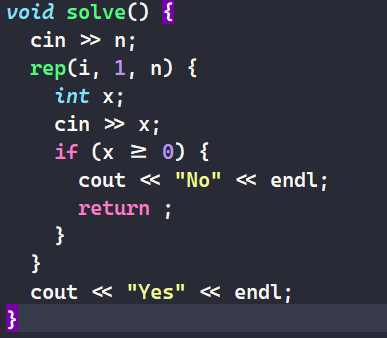
\includegraphics[width=0.7\linewidth]{screenshot001}
			\caption{}
			\label{fig:screenshot001}
		\end{figure}
		
	\end{frame}
	
	\section{B}
	\begin{frame}
		\frametitle{Problem B}
		一共有 $n$ 个球，给出每个球的颜色和大小，让你给出每种颜色的球的最大大小
		\begin{itemize}
			\item<1-> 以颜色映射大小使用桶数组，在输入颜色时将桶数组为该输入颜色的大小与输入的大小去 $max$ 即 $to[c[i]] = max(to[c[i]], s[i])$
			\item<2-> \begin{figure}
				\centering
				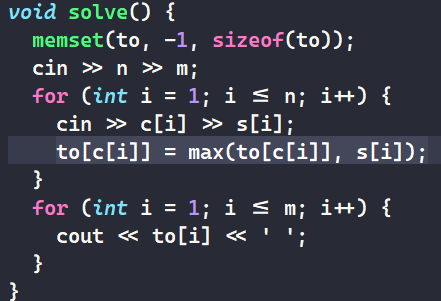
\includegraphics[width=0.7\linewidth]{screenshot002}
				\caption{}
				\label{fig:screenshot002}
			\end{figure}
			
		\end{itemize}
	\end{frame}
	
	\section{C}
	\begin{frame}
		\frametitle{C}
		交互题，给出 $n$ 个点在数轴上，你可以提问 $i$ 与 $j$ 两个点之间的距离是否小于等于 $1$，并在 $2n$ 次询问中得到该数轴上距离小于等于 $1$ 的个数
		\begin{itemize}
			\item<1-> 点从左到右排列，距离随 $j$ 单调递增
			\item<2-> 用双指针维护窗口 $[l, r]$
			\item<3-> $r$ 只增不减，总查询 $O(N)$
			\item<4-> 答案 $= \sum_{i=1}^{N} (R_i - i)$
		\end{itemize}
	\end{frame}
	\begin{frame}
		\begin{itemize}
			\item<1-> 如何求 $R_i$ 呢
			\item<2-> 以 $i$ 作为 $l$ 与 $r$ 构成区间，并循环查询区间长度是否小于等于 $1$，在查询失败前一个节点即为 $r$ 的最大值
			\item<3-> 即代码为\begin{figure}
				\centering
				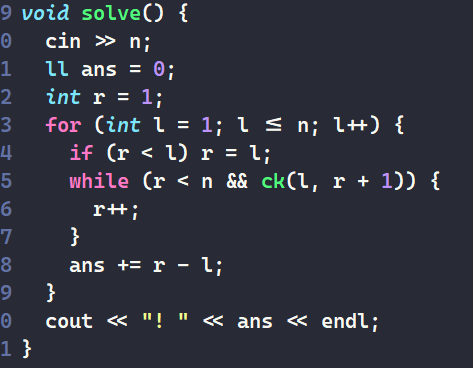
\includegraphics[width=0.7\linewidth]{screenshot003}
				\caption{}
				\label{fig:screenshot003}
			\end{figure}
			在这里的 $ck()$ 是值询问点 $l$ 与点 $r$ 的距离
		\end{itemize}
	\end{frame}
	
	\section{D}
	\begin{frame}
		有一个 $N*N$ 的 Grid，进行 $M$ 次操作，每一次操作分别是删除第$r_i$行所有旗子与删除第$c_i$ 行所有旗子，随后在 $(r_i, c_i)$ 放置旗子
		\begin{itemize}
			\item<1> 我们可以转换成一个数学问题，维护两个分别为行和列的集合，我们命名他们为 $S_r	$ 与 $S_c$
			$S_{\text{r}} = \{ r \mid \text{第 } r \text{ 行在 } i \text{ 之后被删除过} \}$ \\
			$S_{\text{c}} = \{ c \mid \text{第 } c \text{ 列在 } i \text{ 之后被删除过} \}$
			\item<2-> 我们可以有一个很方便的维护，若 $R_i \notin S_{\text{r}}$ 且 $C_i \notin S_{\text{c}}$，则棋子保留，$ans++$
			\item<3> tips: 需要倒序操作，因为如果从前往后维护集合无法预判接下来是否会有删除操作关联本次操作
		\end{itemize}
	\end{frame}
	
	\section{E}
	\begin{frame}
		有 $N$ 幅卡片，正背面分别写着数字 $A$ 与 $B$，你有 $k$ 次机会翻转 $[l, r]$ 区间的卡片，求最终朝上的数字总和的最大值。
		\begin{itemize}
			\item<1-> 考虑 dp 做法求翻转可得收益
			\item<2> 我们设 $dp[i][j]$ 为当前处理到第 $i$ 个位置，翻转了 $j$ 次有最大收益
			\item<3> 枚举 $i \in [1, n]$，每次枚举有两种决策方案
			
			\begin{itemize}
				\item 1：不以 $i$ 结尾翻转任何区间
				\[
				dp[i][j] = dp[i-1][j]
				\]
				
				\item 2：以 $i$ 结尾翻转一个区间 $[l, i]$
				\[
				dp[i][j] = \max_{1 \le l \le i} \left( dp[l-1][j-1] + \sum_{x=l}^{i} (B_x - A_x) \right)
				\]
			\end{itemize}
			
			\item<4> 用前缀和与差分数组优化，即可将 $\sum_{x=l}^{i} (B_x - A_x)$ 操作复杂度优化到 $O(1) $
			\item{5} 后面再加上初始正面朝上的总和即可获得题目要求的答案
		\end{itemize}
	\end{frame}
	\begin{frame}
		\begin{figure}
			\centering
			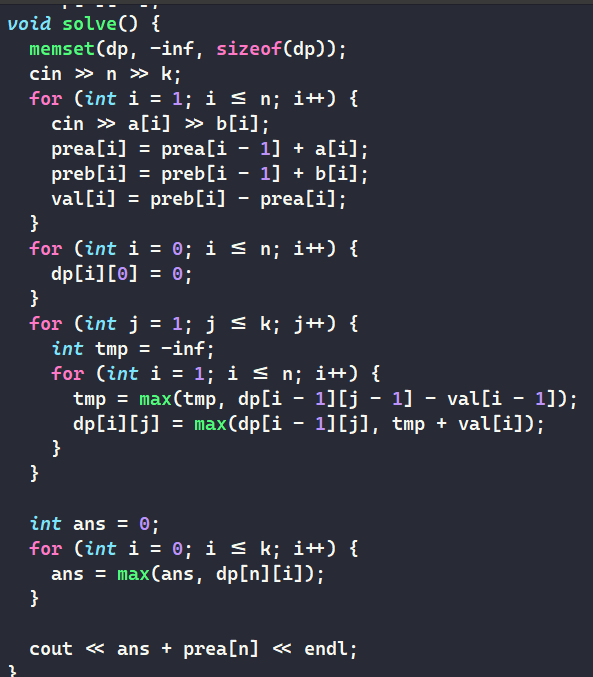
\includegraphics[width=0.7\linewidth]{screenshot004}
			\caption{}
			\label{fig:screenshot004}
		\end{figure}
		
	\end{frame}
	
	\section{?}
	\begin{frame}
		\begin{figure}
			\centering
			\includegraphics[width=0.7\linewidth]{C:/Users/guozi/AppData/Local/Temp/QQ_1783780343150}
			\caption{}
			\label{fig:qq1783780343150}
		\end{figure}
		
	\end{frame}
		
\end{document}